\clearpage \subsection{Exploration}

\label{chap:data_exploration}

As already mentioned in the previous section, two data sets exist which can be interpreted. First, this section examines all features that are present in both datasets. Finally, the different features are examined to finally decide on a dataset to be used for the models. 

The following table describes all the features that appear throughout the datasets, their description, and datatype. In \emph{Python}, \emph{Strings} are stored as objects.

\begin{table}[H]
    \caption{Overview of Features and their Dataype}
    \label{tab:overview-features}
    \resizebox{\textwidth}{!}{%
    \begin{tabular}{@{}ccl@{}}
    \toprule
    \textbf{Feature} & \textbf{Datatype} & \textbf{Description}                                     \\ \midrule
    name                & object    & name of a player                                              \\
    position            & object    & position of a player, i.e. goalkepper, attacker               \\
    matchday            & int64     & matchday where the results happened, i.e. 1, 2, 34            \\
    team\_name          & object    & name of the team in which the player competes                 \\
    is\_home            & bool      & boolean indicating whether the game was played at home or not \\
    odds\_win           & float64   & odds for the team to win                                      \\
    odds\_draw          & float64   & odds for the team to draw                                     \\
    odds\_lose          & float64   & odds for the team to lose                                     \\
    event\_type         & object    & event type, i.e. goal, pass, unsuccessfullTackle              \\
    occurrences         & int64     & number of occurences of event\_type for this matchday          \\
    performance\_trend  & int64     & recent performance trend for a player                         \\
    score               & int64     & individual player score S\textsubscript{P\textsubscript{i}}  \\\bottomrule
    \end{tabular}%
    }
\end{table}

Each feature is first analyzed individually and then in combination with each other. This analysis is mainly done in the order of the table, starting with the dataset containing event types and their occurrences.

\subsubsection{Name}

The name of a player is synonymous with the player itself in this context. As can be seen from the following figure, there aren't identical numbers of entries for each player. This deviation should not be the case because, in the previous section, an entry was assigned to each player for each matchday and event type. The reason for this difference is that there are entries for the event types \textbf{player\_on} and \textbf{player\_off} in the data set, which is not found in the points catalog from SPITCH and has no influence on the score. For this reason, these events can be ignored.

\begin{figure}[H]
    \centering
    \label{fig:distribution_of_events_per_player}
    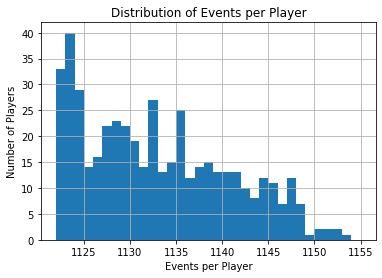
\includegraphics[width=10cm]{chapter/4_implementation/section/2_data/section/figures/distribution_of_events_per_player.png}
    \captionsetup{justification=centering}
    \caption{Distribution of Events per Player}
\end{figure}

After deleting the two event types mentioned above from the data set, there are \numprint{1122} rows for each of the 467 players. This is equivalent to 33 different event types on 34 matchdays. Therefore, the data set has a total of \numprint{1122} rows times 467 players, i.e. \numprint{523974} entries. 

 \clearpage \subsubsection{Matchday, Event Type, and Home Advantage}

Accordingly to the calculation from the previous section, for each matchday, there are 33 event types times 467 players, i.e., \numprint{15411} rows, and for each event type, there are 34 matchdays times 467 players, \numprint{15878} entries. Since in the German \emph{Bundesliga} every team plays every team twice, once at home and once away, there are precisely the same number of rows for matches played at home and matches played away.

\subsubsection{Position}

From the figure \ref{fig:number_of_players_per_position} below, it can be seen that there are four different positions in the dataset, with the midfielder being the most common position with 193 entries out of 467 (41.3\%) and goalkeeper being the rarest position with 35 entries (7.5\%). This distribution is reasonable given that most formations have more midfielders than any other position, and there is always only one goalkeeper.

\begin{figure}[H]
    \centering
    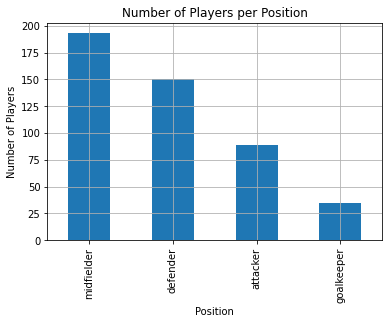
\includegraphics[width=9cm]{chapter/4_implementation/section/2_data/section/figures/number_of_players_per_position.png}
    \captionsetup{justification=centering}
    \caption{Number of Players per Position}
    \label{fig:number_of_players_per_position}
\end{figure}

\subsubsection{Team Name}

\begin{figure}[H]
    \centering
    \label{fig:numer_of_players_per_team}
    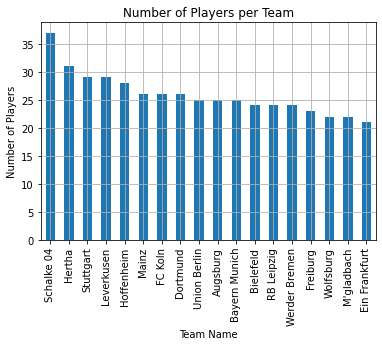
\includegraphics[width=10cm]{chapter/4_implementation/section/2_data/section/figures/number_of_players_per_team.png}
    \captionsetup{justification=centering}
    \caption{Number of Players per Team}
\end{figure}

The figure shows that Eintracht Frankfurt has the fewest players with 21. Schalke 04 has the most players with 37. The average number of players per team is 25.

\subsubsection{Betting Odds}

Many different betting odds systems exist. The betting odds used in this thesis follow the most popular model. In this model, the betting odds represent the factor by which the stake is multiplied if the event on which the bet was placed occurs. Through this system, bets can be placed on any game outcome with a chance of winning. The more probable the outcome, the lower the factor. This factor is influenced by various aspects such as the assumed playing strength of the teams, but also how many bettors have already bet on this outcome. Since every bookmaker has its own methods for this calculation, an average of 13 different platforms is chosen. This betting odds model has the advantage that it is lucrative for the bookmaker in every case, as he chooses the factors in such a way that no matter what the outcome of the match, the stakes paid in exceed the profit to be cashed out. For this reason, these betting odds should be assessed with caution. However, they represent a relatively general and, above all, up-to-date picture of the teams' probabilities of winning. The figure below shows that the betting odds are mostly in the range between two and four for winning or losing. Anything above or below that range indicates a one-sided game. Here, 24.69 has been the maximum value, and the corresponding counterpart 1.09 was the minimum value. While the range for a draw is smaller, the factor itself is higher in general.

\begin{figure}[H]
    \centering
    \label{fig:distribution_of_betting_odds}
    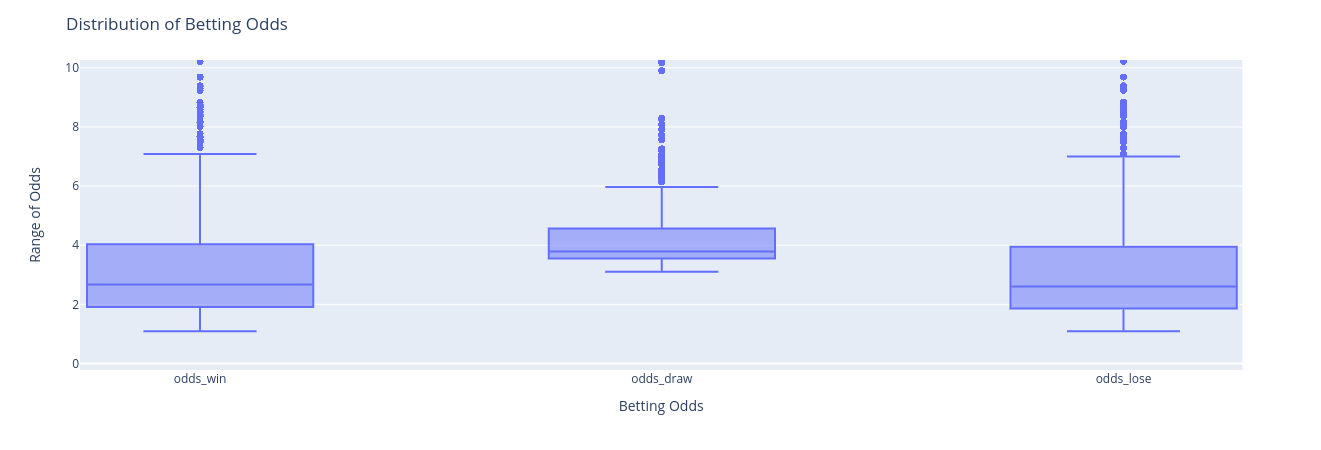
\includegraphics[width=16.5cm]{chapter/4_implementation/section/2_data/section/figures/distribution_of_betting_odds.png}
    \captionsetup{justification=centering}
    \caption{Distribution of Betting Odds}
\end{figure}

\subsubsection{Occurences}

The bar chart below shows that most of the rows have a value of 0 (\textbf{87.3\%}). The frequency monotonically decreases as one moves further away from zero. Therefore, the main task of machine learning models would be to predict situations where the result are not zero, which leads to a classification problem instead of the initial regression problem. As announced at the beginning of the section, a final decision has to be made in favor of one data set. In addition to the figure below, further investigations with this dataset, which cannot be presented in this thesis due to the large volume, showed that its use is unsuitable. For this reason, it was decided to use the data set that contains the calculated scores.

\begin{figure}[H]
    \centering
    \label{fig:percentage_distribution_of_occurrences}
    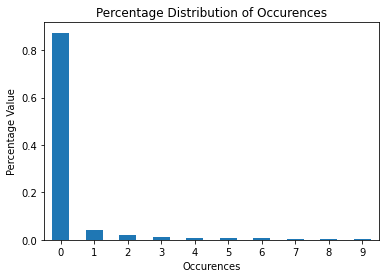
\includegraphics[width=7.5cm]{chapter/4_implementation/section/2_data/section/figures/percentage_distribution_of_occurences.png}
    \captionsetup{justification=centering}
    \caption{Percentage Distribution of Occurences}
\end{figure}

\subsubsection{Score}

An interesting statistic in relation to the score, especially about the significance of the performance trend, is the autocorrelation. The autocorrelation indicates the extent to which previous values are predictive of future values of the same feature. Figure \ref{fig:autocorrelation_score} shows an autocorrelation between 0.65 and 0.7 for the lags between -10 and 10. Additionally, the correlation slowly decreases as one moves further away from the actual value. This small decrease indicates that more current values give better predictions than past values. This conclusion confirms the choice of exponential moving averages for the calculation of the performance trend. Overall, an autocorrelation of 0.7 indicates a medium to strong relationship between past and current values.

\begin{figure}[H]
    \centering
    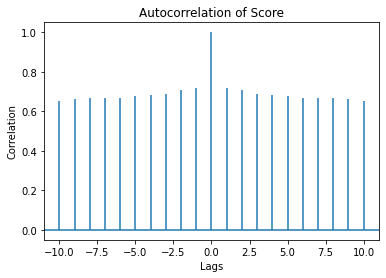
\includegraphics[width=8cm]{chapter/4_implementation/section/2_data/section/figures/autocorrelation_score.png}
    \captionsetup{justification=centering}
    \caption{Autocorrelation of Score}
    \label{fig:autocorrelation_score}
\end{figure}

Looking at the score, two groups of players are particularly interesting. The first group consists of players who rarely score many points and are consequently not drafted by many managers. The second group consists of players who score relatively confidently. The players in this group are, therefore, probably the most expensive because many managers draft them. Two different approaches are taken in the analysis of the data to separate the players in these two groups. To begin with, the players who belong to the first group will be examined by looking for the players with the highest average of points per game. Secondly, it is examined which players have scored the most points overall over the entire season. These are the players in the second group.


\begin{figure}[H]
    \centering
    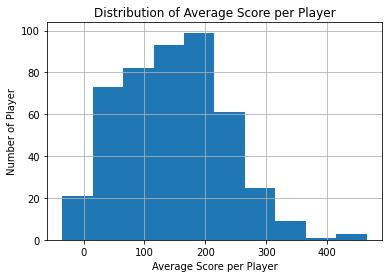
\includegraphics[width=8cm]{chapter/4_implementation/section/2_data/section/figures/distribution_of_average_score_per_player.png}
    \captionsetup{justification=centering}
    \caption{Distribution of Average Score per Player}
    \label{fig:distribution_of_average_score_per_player}
\end{figure}

Figure \ref{fig:distribution_of_average_score_per_player} shows the distribution of the average scores of all players. This figure indicates that most players receive an average score of around 200. There exists a small group of players who achieve an average score of over 300. Interestingly, more players achieve more than 400 points than players who achieve between 350 and 400 points.

\begin{figure}[H]
    \centering
    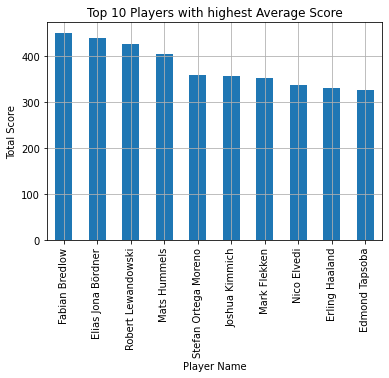
\includegraphics[width=8cm]{chapter/4_implementation/section/2_data/section/figures/top_10_player_average_score.png}
    \captionsetup{justification=centering}
    \caption{Top 10 Players with highest Average Score}
    \label{fig:top_10_player_average_score}
\end{figure}

The above figure displays the ten players with the best average score. Surprisingly, many players in this group are not well-known and therefore inexpensive. These are the players who need to be ideally lined up by the model because, on the one hand, they score a lot of points and, on the other, their low transfer market value means they don't have to earn a lot of points to be valuable. Nevertheless, there are also very well-known players, such as \emph{Mats Hummels} or \emph{Robert Lewandowski}. With these players, the models have to weigh up whether to put them in the line-up or not, as their high transfer market value means that they have to earn a lot of points first in order to recoup the manager points they have cost. These players are especially worth choosing as captain because the points scored are doubled, but their transfer market value deduction is not.

Regarding the second group of players, figure \ref{fig:distribution_of_total_score_per_player} shows that there are many players who have scored between zero and \numprint{1000} points throughout the season. Given this and the prior observations, it can be concluded that many players in the data set are rarely fielded, but when they are fielded, they still achieve an average score.

\begin{figure}[H]
    \centering
    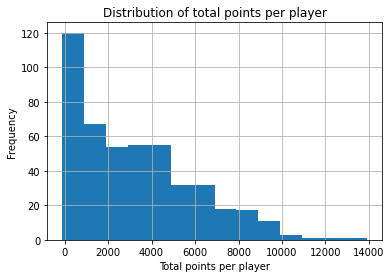
\includegraphics[width=8cm]{chapter/4_implementation/section/2_data/section/figures/distribution_of_total_score_per_player.png}
    \captionsetup{justification=centering}
    \caption{Distribution of Total Score per Player}
    \label{fig:distribution_of_total_score_per_player}
\end{figure}

On the other end of the axis, there is only a small number of extraordinary players who scored over \numprint{10000} points throughout the season. These players have two characteristics: they are fielded often and score confidently. The following figure shows the Top 10 players regarding the total score over the entire season. 

\begin{figure}[H]
    \centering
    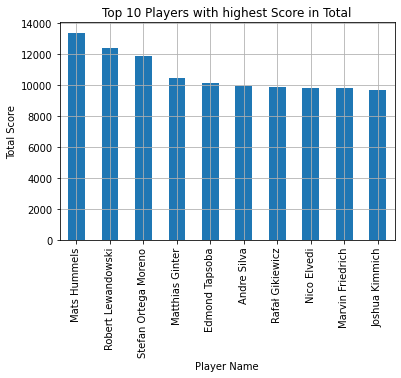
\includegraphics[width=8cm]{chapter/4_implementation/section/2_data/section/figures/top_10_player_total_score.png}
    \captionsetup{justification=centering}
    \caption{Top 10 Players with highest Total Score}
    \label{fig:top_10_player_total_score}
\end{figure}

In contrast to the previous group, this top 10 contains many well-known players, once again including \emph{Mats Hummels} and \emph{Robert Lewandowski} at the front positions.

\subsubsection{Correlation between position and score}

Interestingly, all positions are represented in the previous figure \ref{fig:top_10_player_total_score}. For this reason, further insights into the correlation between the position and the scores are provided in this paragraph. The figure \ref{fig:average_score_per_position} shows that goalkeepers score the most points on average, followed by defenders and midfielders. Attackers score the fewest points. This finding is counterintuitive as goals are scored highest in SPITCH and most goals are scored by attackers. It can be deduced from this finding that it often depends on many small events, such as passing or taking the ball away, to achieve a high score. 

Furthermore, conclusions for the formation can be drawn from this diagram. For example, if goalkeepers score the most points on average, it might be a good strategy to choose the goalkeeper as captain. In addition, a defensive formation should be chosen, as defenders and midfielders score more points on average than attackers. 

\begin{figure}[H]
    \centering
    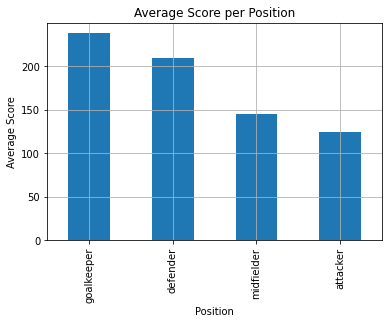
\includegraphics[width=9cm]{chapter/4_implementation/section/2_data/section/figures/average_score_per_position.png}
    \captionsetup{justification=centering}
    \caption{Average Score per Position}
    \label{fig:average_score_per_position}
\end{figure}

The following two data explorations are carried out exclusively with the Betting Odds CSV data set \parencite[][]{football-data_germany_nodate} and should therefore be considered separately from the previous data set.

\subsubsection{Correlation between Betting Odds and Match Result}

This section aims to examine the influence betting odds have in the prediction of future player performance. For this reason, the match result is taken from the CSV in addition to the betting odds. First, the percentage of cases in which betting odds predicted the correct final result is examined. Therefore, the delta between the odds for the home and away team is calculated. From the previous investigations of the betting odds, it is known that when the odds for a draw are highest, the odds for the home and away team usually differ by a maximum of 0.5. For this reason, a draw is expected for a delta of less than 0.5. Otherwise, a win is expected for the team with lower odds. When this procedure is applied to the entire data set, the betting odds predict the correct outcome \textbf{53.6\%} of the time. This result is a remarkable 21\% difference to the probability of one-third if one had to guess the result. Thus, this study concludes that betting odds are indicative of which team is likely to win. 

\begin{figure}[H]
    \centering
    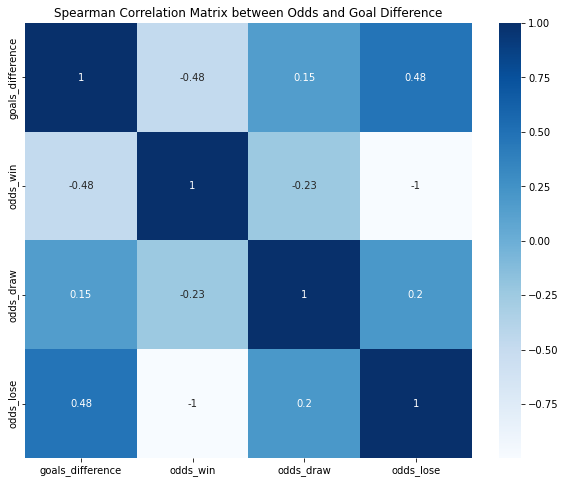
\includegraphics[width=10cm]{chapter/4_implementation/section/2_data/section/figures/correlation_matrix_odds_goal_diff.png}
    \captionsetup{justification=centering}
    \caption{Spearman Correlation Matrix between Odds and Goal Difference}
    \label{fig:correlation_matrix_odds_goal_diff}
\end{figure}

However, the game of SPITCH is more complex than just predicting the winning team. It would also be interesting to know whether betting odds can also predict the level of victory or defeat. Because teams that are expected to win higher than others consequently score more goals, which leads to higher scores. In order to prove this influence, the final goal difference is computed. Afterward, the correlation between this variable and the betting odds is calculated using \emph{Spearman's rank correlation coefficient}. The correlation matrix in figure \ref{fig:correlation_matrix_odds_goal_diff} indicates a medium correlation of 0.48 or -0.48 respectively between the goal difference and the odds for winning or losing. Accordingly, the betting odds not only allow to predict which team is likely to win but also to estimate with a certain degree of accuracy how clear the result will be. 

\subsubsection{Home advantage}

The literature review showed that home advantage had been used in many models written to predict sports outcomes. In the data set used for the models in this thesis, a column regarding the home advantage was also added. The following figure shows that home advantage also played a role in the 2020/2021 season. From the perspective of the home team, 42\% of the matches were won and 31\% lost. 

\begin{figure}[H]
    \centering
    \label{fig:home_advantage}
    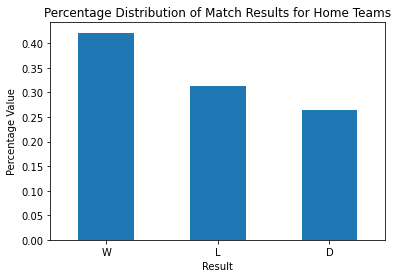
\includegraphics[width=7.5cm]{chapter/4_implementation/section/2_data/section/figures/home_advantage.png}
    \captionsetup{justification=centering}
    \caption{Percentage Distribution of Match Results for Home Teams}
\end{figure}